%% The following is a directive for TeXShop to indicate the main file
%%!TEX root = diss.tex

\chapter{The \toolname{} Plugin}
\label{ch:Tool}

% TODO: typeset the following nicely.
% \begin{epigraph}
%   \emph{What information consumes is rather obvious: it 
%     consumes the attention of its recipients.
%     Hence a wealth of information creates a poverty of attention, and a need 
%     to allocate that attention efficiently among the overabundance 
%     of information sources that might consume it.}
%      ---~Herbert A. Simon
% \end{epigraph}

\noindent \toolname{} is an open-source\footnote{\url{https://github.com/jyoo980/reach-hover}}
plugin developed on the JetBrains IntelliJ Platform.
Section \ref{sec:DesignMeth} discusses the design methodology for \toolname{},
derived from the data presented in Chapter \ref{ch:Survey} and an investigation
of the current tools that provide information that might be used to help answer
reachability questions.
In section \ref{sec:UsingReachHover}, we describe how a user might use
\toolname{} in a software development scenario, with a particular focus on
its mechanism of invocation and how it visualizes data.
The implementation of \toolname{} is detailed in section
\ref{sec:Impl}.

\section{Design Methodology}
\label{sec:DesignMeth}

\noindent To inform the design of \toolname{}, we analyzed the data from a 
survey that sought to identify the type and frequency of reachability questions 
that are asked by software developers in practice.

Figure \ref{fig:SurveyResults} shows that Development Questions 1, 2, 5, and 9
were the most frequently asked among our respondents.
Using Table \ref{Table:SurveyTags} to map these questions to their associated
tags, we found that $Q_{find}$ was the most frequent type of question asked out
of the top four ranked by our respondents.
Specifically, these questions were:

\begin{itemize}
  \item[] \textbf{Development Question 1}:\\ \textit{Where did a value come from,
  and/or how was it formed?}
  \item[] \textbf{Development Question 2}:\\ \textit{Given some data, which
  parts of it are modified downstream?}
\end{itemize}

\par We noted that these questions are thematically related. They are instantiations 
of the \textit{find} category of reachability question, and they can also be
answered by traversing backward and forward in a data-flow trace, respectively.
For example, to answer Development Question 1, a user could invoke a backward
data-flow trace, and filter for nodes that have a control or data dependency
on the value under analysis.
To answer Development Question 2, a forward data-flow analysis can be invoked,
and the result can be filtered for control or data dependencies on the value
under analysis.
Consequently, we decided to build \toolname{} with a particular focus on
supporting these two questions for the sake of thematic coherence.

\par Since information provided from a data-flow trace could be used to answer
the questions we attempt to support with \toolname{}, we began by investigating 
existing data-flow analysis tools to obtain an understanding of the current 
landscape of analysis tooling.
The IntelliJ IDEA \ac{IDE} exposes forward and backward data-flow analysis
capabilities to users.
Figure \ref{fig:IntelliJDataflow} shows how a user might invoke a backward 
data-flow analysis, while the result of this analysis is shown in
Figure \ref{fig:IntelliJDataflowResult}.
We found these pre-existing data-flow capabilities to be a good basis for the 
development of \toolname{} due to its ease of extension via the JetBrains 
IntelliJ Platform \ac{SDK}.

\par Next, we began to identify pain points that users might face as they
invoked the data-flow analysis tool.
We observed that discovering the tool itself might be difficult for
users; the action to invoke the tool was a three-click action.
Additionally, the action was hidden behind a context menu that did not appear
to have a strong information scent that guided users to discovering and invoking
the tool from a very broad list of options (\ie data-flow-specific analyses
are accessed via a general ``Analyze" menu element).
In the result presented by the data-flow analysis tool, each element in the 
data-flow trace is presented as an node in a tree-like structure that is 
structually similar to a conventional hierarchical tree.
We found this to be useful for preserving the structural information relevant
to our target reachability questions (\eg method calls \texttt{a}, and \texttt{b}
within a method \texttt{c} are displayed as children of the node \texttt{c} in
the tree).

\par Although structural information was easily preserved through the tree, each node
displayed only the single line of code within the data-flow trace, often
without visual aids such as syntax highlighting.
This meant that users often analyzed each node in isolation from any surrounding
context, particularly if they were not aware that double-clicking a node in the
tree would focus the editor pane to the line of code under inspection.
However, this might introduce the additional problem of frequent context
switching and reconstruction as editor focus shifts between files and code
blocks.

\par Investigating the current tooling available for data-flow analysis, and
its associated user pain points provided a foundation for the design of 
\toolname{}.
We attempted to achieve the following with the design of our tool:

\begin{itemize}
  \item[] \textbf{Design Goal 1}: \\
    \textit{
      User friction should be minimized between the developer and \toolname{},
      especially with respect to how they might discover and invoke the tool.
    }
  \item[] \textbf{Design Goal 2}: \\
  \textit{
    \toolname{} should present more context surrounding a data-flow node in
      a way that minimizes the amount of context switching for a developer.
  }
\end{itemize}

We describe the user-facing result of implementing these goals in section
\ref{sec:UsingReachHover}, while a technical discussion of their implementation 
is discussed in section \ref{sec:Impl}.

\section{Using \toolname{}}
\label{sec:UsingReachHover}

In this section, we describe how a user might interact with \toolname{}, framed
within the context of a software development task.
First, we describe how a user might invoke our tool to begin the process
of answering a reachability question.
Next, we describe the user interface of the visualization presented by 
\toolname{}.

\subsection{Invocation Interaction}
\label{subsection:InvocationInteraction}

TODO: say some shit here...

\begin{figure}[ht]
\centering
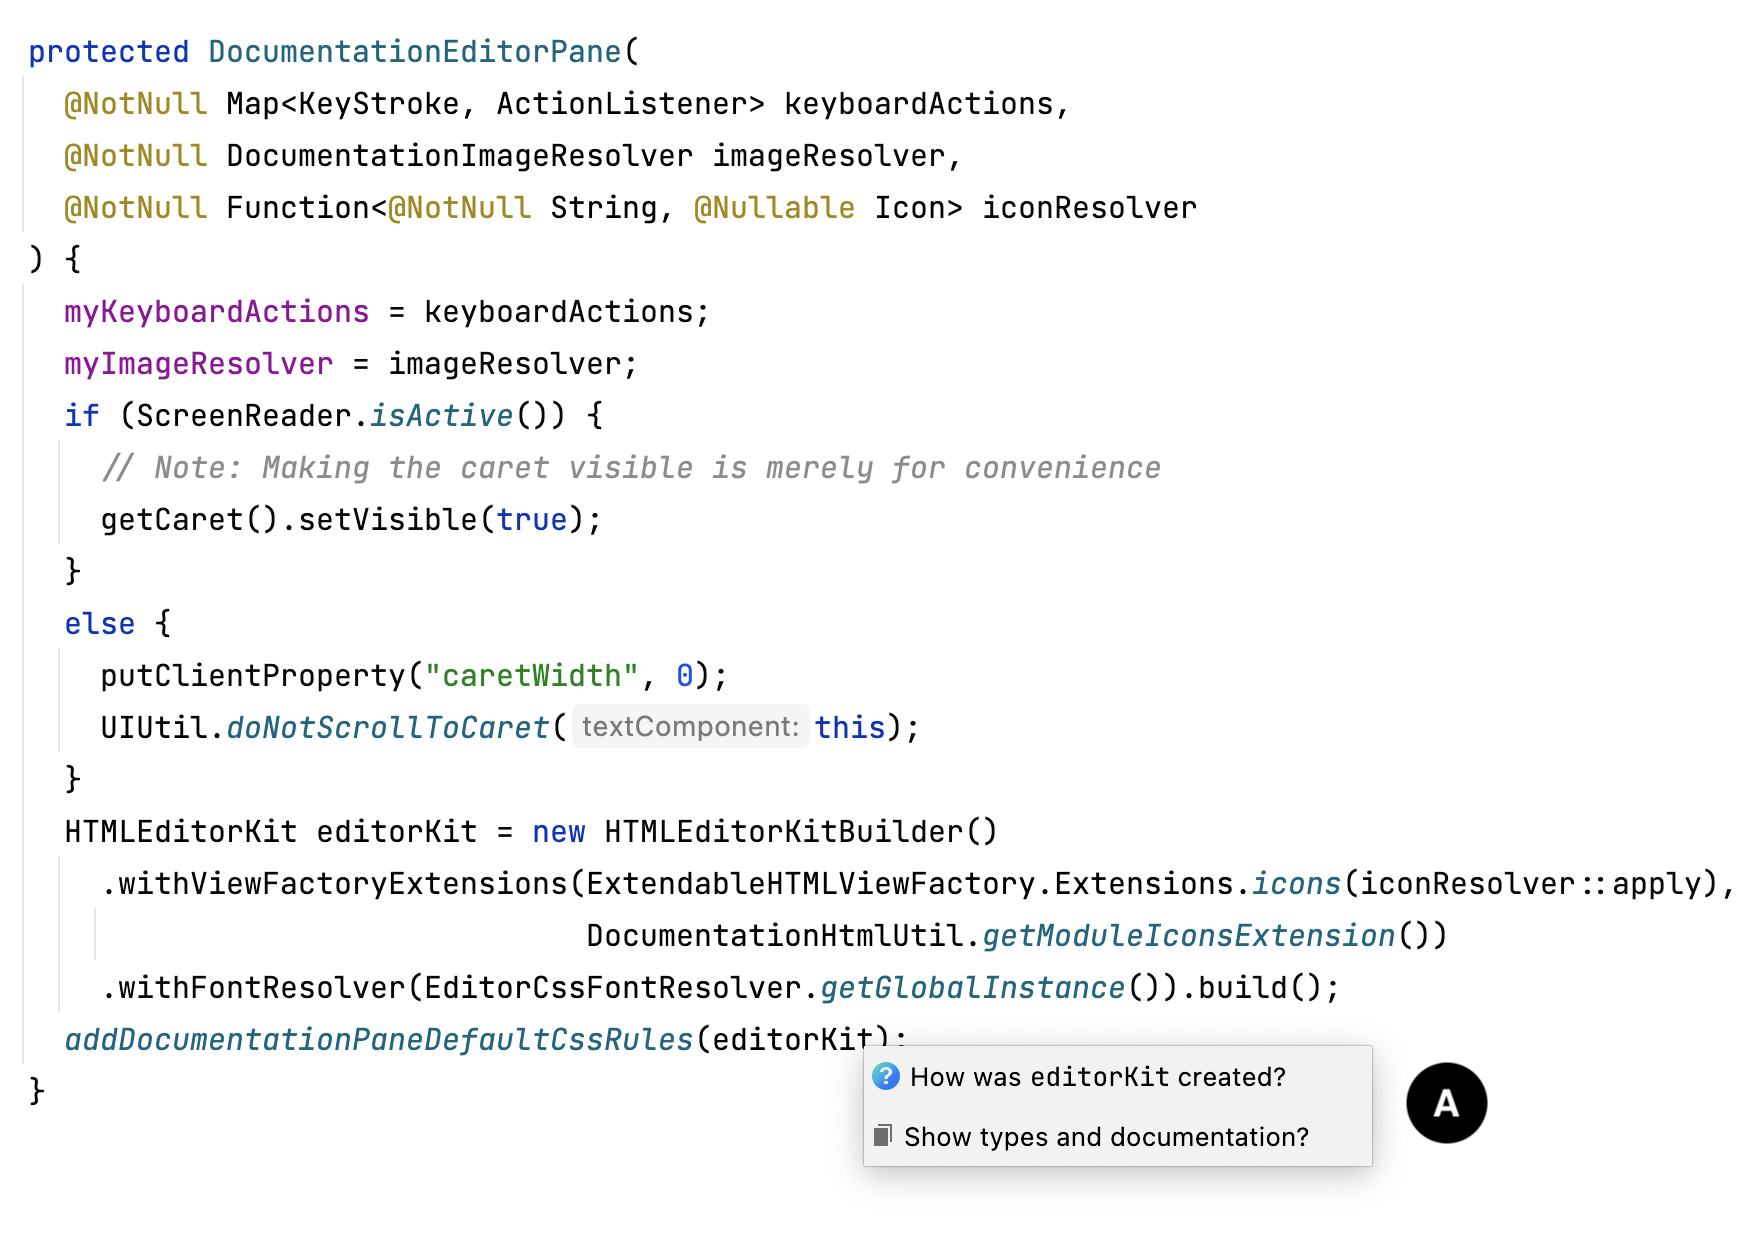
\includegraphics[width=\textwidth]{./figs/reach-hover-invoke.png}
\caption{
  Blah
}
\label{fig:ReachHoverInvoke}
\end{figure}


\subsection{Result Visualization}
\label{subsection:ResultVisualization}

\noindent A goal of \toolname{} was to present more context surrounding the 
result of a data-flow analysis. 
We also wanted to preserve the structural information that was
already provided by existing static analysis tools, such as the data-flow
analysis tooling built into IntelliJ IDEA, or the call hierarchy explorer in
the Eclipse \ac{IDE}, which presents results using the same hierarchical
tree paradigm.

\par Preserving the presentation of structural information served two purposes.
First, we did not aim to completely redesign an interface for viewing data-flow
information;
our goal was to enrich an existing interface with additional information.
Introducing a completely new user interface paradigm might have introduced
additional complexity in the form of developers having to adapt to a new 
paradigm before our tool became useful to them.
Second, we wanted to preserve non-local context, \ie information that is not
directly observable from code and its surrounding context, such as how deep
within a call hierarchy a location in code exists.

\par We present the visualization component of \toolname{} in Figure
\ref{fig:ReachHoverVis}.
Information regarding a reachability question is presented in two main
sub-components.
High-level non-local context is provided in the top half of the main component,
which is the same component used by the the original data-flow analysis tool
built into IntelliJ IDEA.
Fine-grained local context is provided by the preview editor sub-component.
A developer is able to begin investigating code from a high-level by selecting
a row in the top component.
This triggers a change in the preview editor to focus on the line of code under
inspection, which is highlighted in its location in the editor.
Additional information, such as the file and project directory in which the
line of code under inspection is located, is presented in the bottom
toolbar of the main component.

\begin{figure}[ht]
\centering
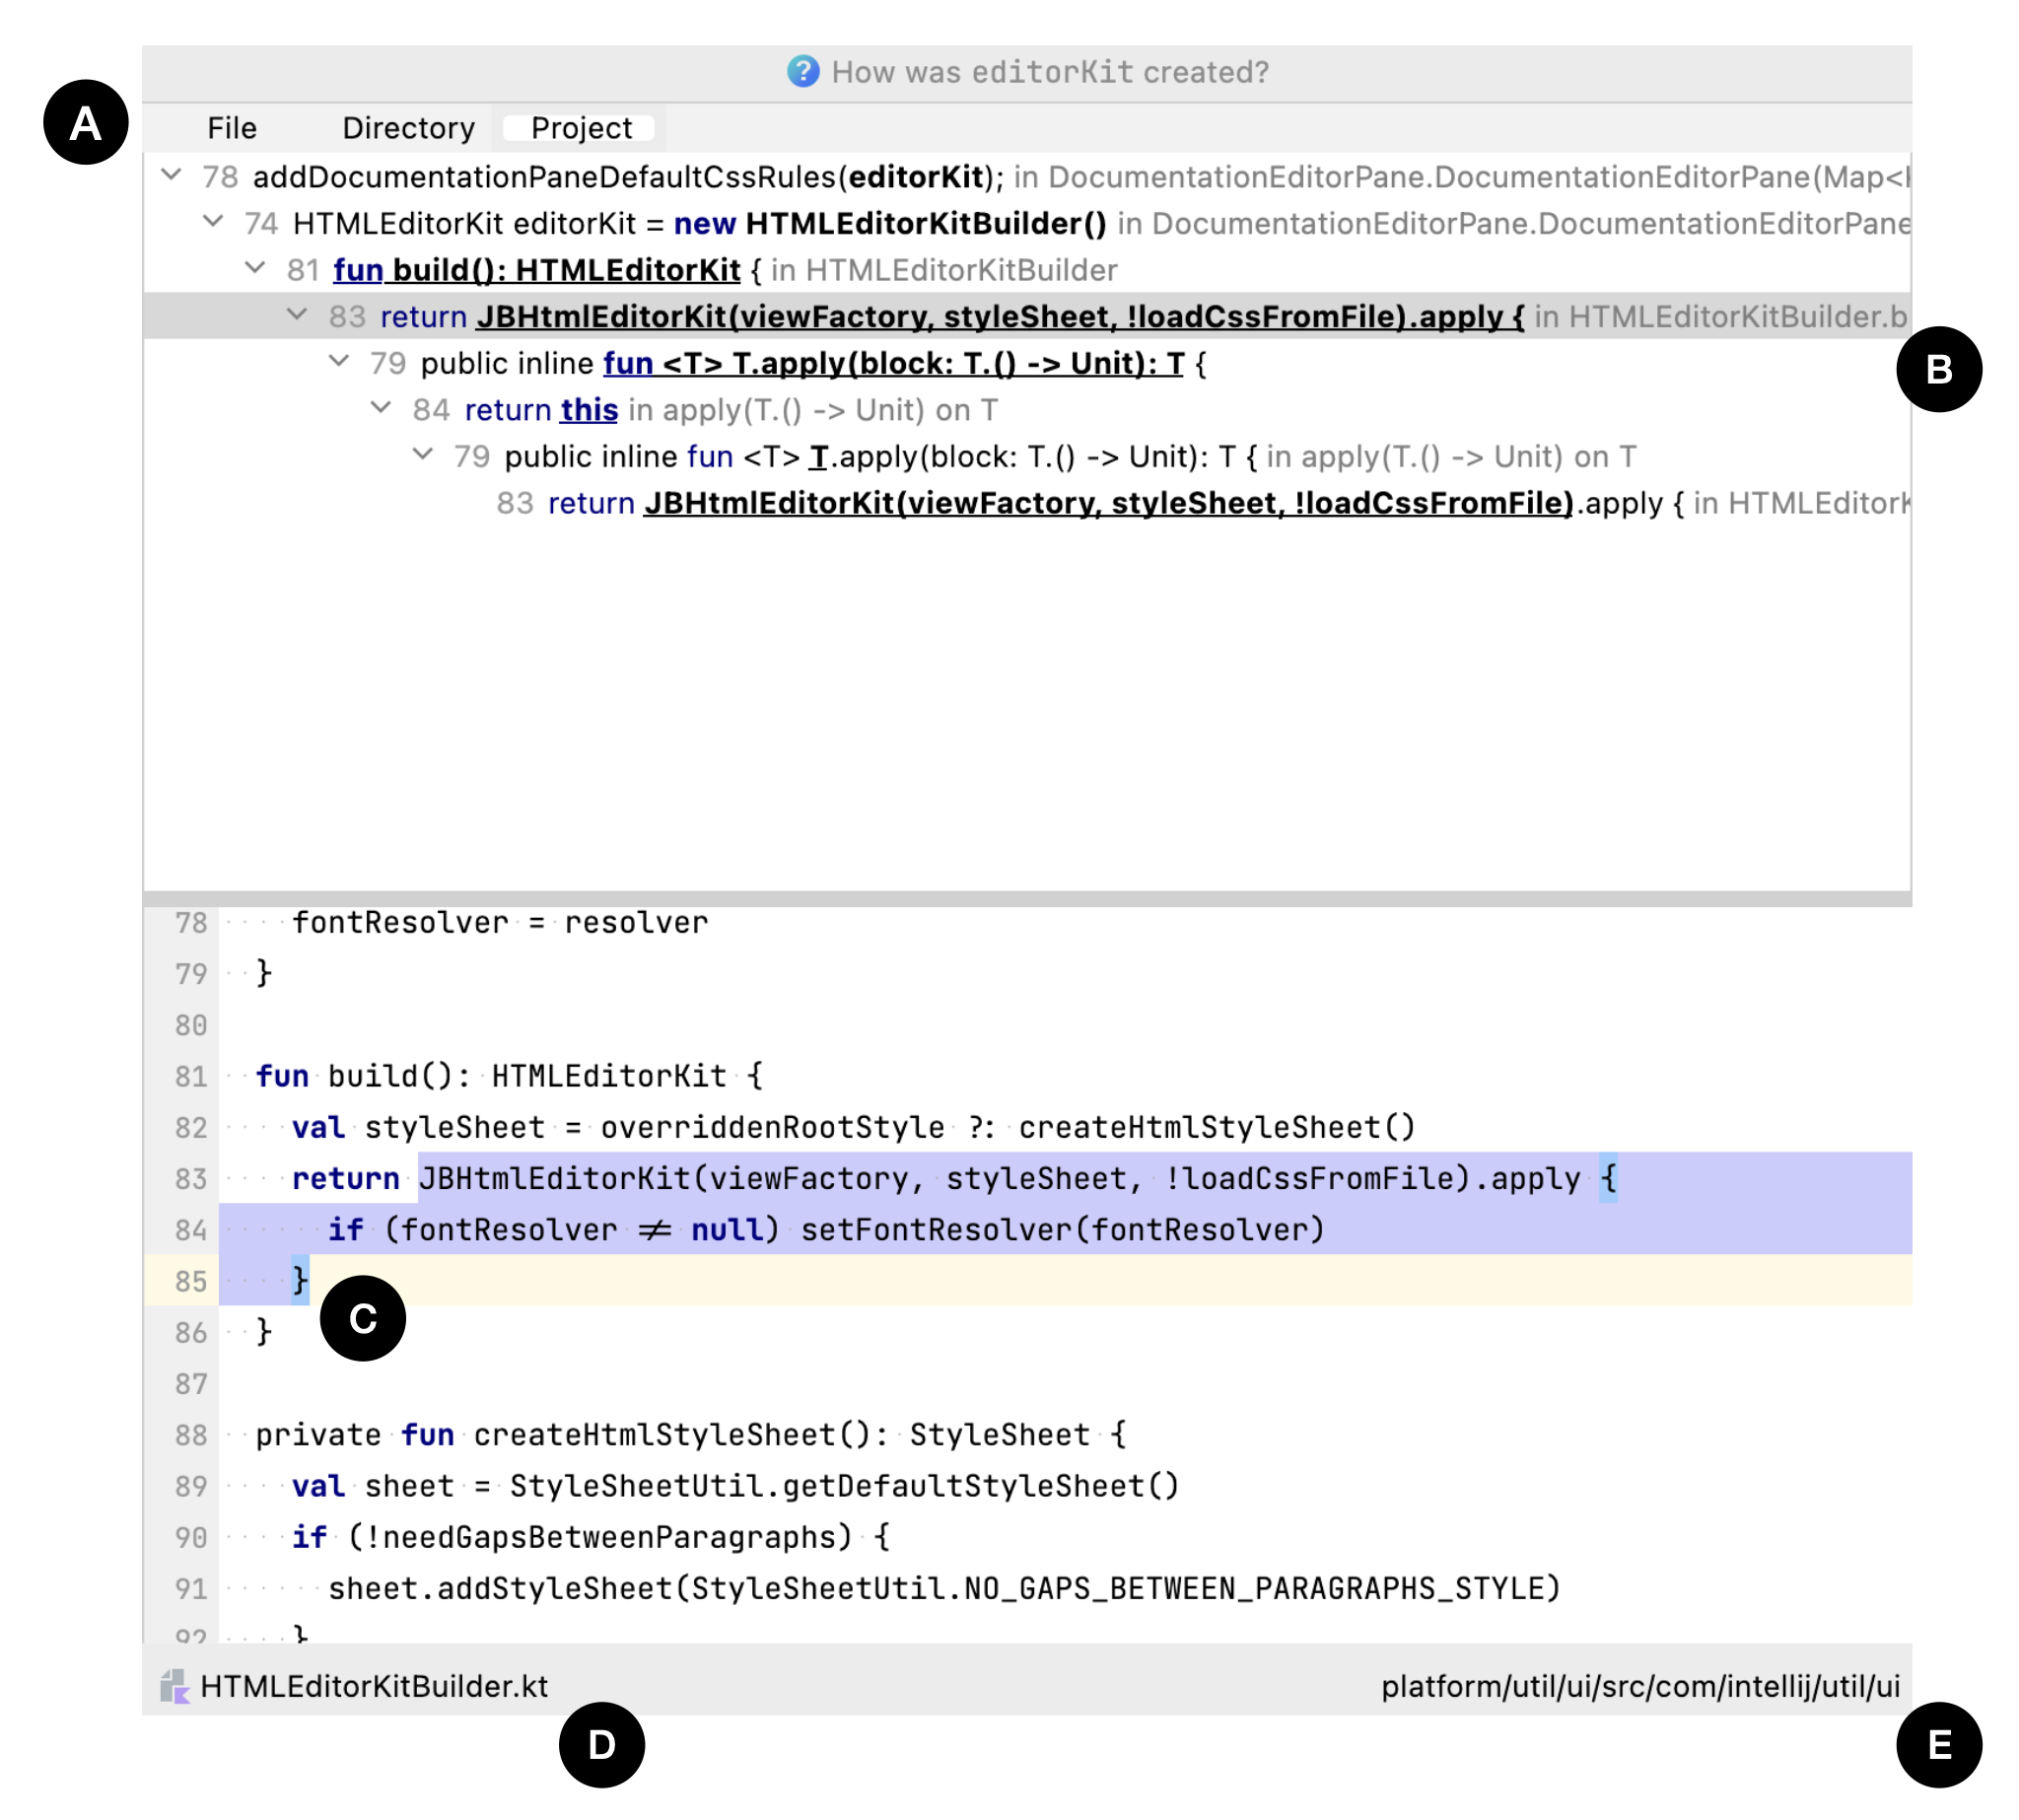
\includegraphics[width=\textwidth]{./figs/reach-hover-vis.png}
\caption{
  A data-flow trace presented by \toolname{}. (A) enables developers to select
  between a file, directory, or project-level scope for the reachability
  analysis. (B) contains the same hierarchical text-tree view as the standard
  IntelliJ data-flow analysis tool. (C) demonstrates the highlighting of the
  code under inspection that corresponds to the selected element in (B).
  The file name and directory are provided by (D) and (E).
}
\label{fig:ReachHoverVis}
\end{figure}

\section{Implementation}
\label{sec:Impl}

\toolname{} is implemented in the Kotlin programming language, and consumes
\acp{API} written in Java that are exposed by the IntelliJ Platform.
The mechanism that reports the viability of the analysis that \toolname{}
exploits to produce a dataflow trace for reachability analysis is 
language-agnostic.
As a result, \toolname{} does not depend on any language-specific syntax to 
determine whether a reachability analysis is viable; it analyzes a genericized 
program syntax tree that is provided by \class{UAST} \dots

\endinput
